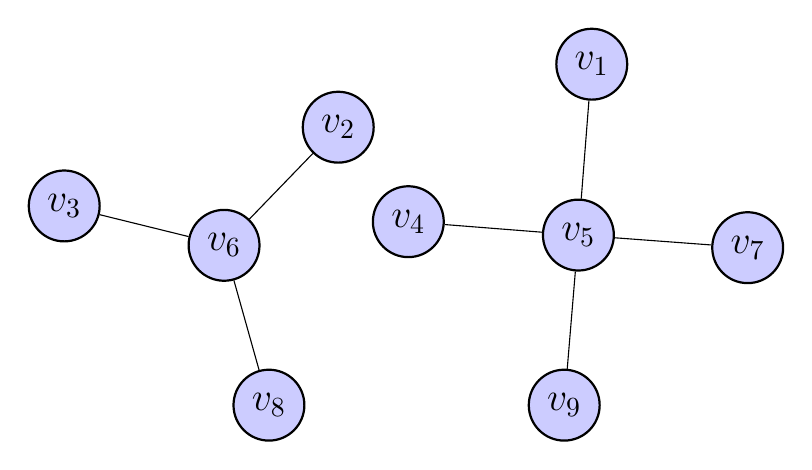
\begin{tikzpicture}[
  scale=1,
  vnode/.style={circle, fill=blue!20, draw=black, thick, minimum size=9mm, inner sep=0pt, font=\Large}
]
  % Vértices
  \node[vnode] (v1) at (7.05, 4.75) {$v_1$};
  \node[vnode] (v2) at (3.83, 3.95) {$v_2$};
  \node[vnode] (v3) at (0.35, 2.95) {$v_3$};
  \node[vnode] (v4) at (4.72, 2.75) {$v_4$};
  \node[vnode] (v5) at (6.88, 2.58) {$v_5$};
  \node[vnode] (v6) at (2.38, 2.45) {$v_6$};
  \node[vnode] (v7) at (9.03, 2.42) {$v_7$};
  \node[vnode] (v8) at (2.95, 0.42) {$v_8$};
  \node[vnode] (v9) at (6.70, 0.42) {$v_9$};

  % Aristas
  \foreach \from/\to in {v1/v5, v2/v6, v3/v6, v4/v5, v5/v7, v5/v9, v6/v8}
    \draw (\from) -- (\to);
\end{tikzpicture}
